\section{Template metaprogramming for Inverse Dynamics}

This work takes its root from the fact that code generated by symbolic formal computation
has in general better performances than generic code for complex robotic models.
This comes for the inner structure of the problem itself. 
For instance, the robot inertia matrix is sparse because the sub-blocks matrices correspond
to the kinematic branches. Then when no coupling exists between some branches, the related sub-blocks mainly is equal to zero.
Formal computation detects such branches and suppresses the related computation.
We are proposing to make the same kind of operations by exploiting C++ template meta-programming.

The result is a template library able to develop an optimized computational tree to 
evaluate the inverse dynamics of a robot class named \textbf{Robot} and to apply it onto the specific instance
named \textbf{robot}, while considering the following complete state $({\bf q}, \dot{\bf q}, \ddot{\bf q})$.
This is obtained by writing the following line:
\begin{verbatim}
rnea< Robot, true >::
  run(robot, q, dq, ddq);
\end{verbatim}
It is template metaprogramming because the code function:
\begin{verbatim}
rnea<Robot,true>::run(robot,q,dq,ddq)
\end{verbatim}
is adapted at compile time to the type \textbf{Robot}. 
During execution, the model specificities are used to update  \textbf{robot}
internal variables according to $(\bf{q},\dot{\bf q},\ddot{\bf q})$.

\subsection{Simple example of functional programming using C++}
A famous example of functional programming in C++ is the factorial computation:
\begin{verbatim}
template <int n>
struct factorial {
 enum { 
   value = n * factorial<n - 1>::value 
 };
};
 
template <>
struct factorial<0> {
	enum { value = 1 };
};
\end{verbatim}
At compile time, when the compiler finds  \begin{verbatim}factorial<4>\end{verbatim}
it directly computes $24$ by successive substitutions.
The same type of mechanism is used to develop the RNEA algorithm from the model \textbf{Robot}.
In order to achieve a decoupling between the model and the robot instances \softmetapod is using 
a template based container proposed by boost::fusion
which allows an array like syntax with templates \footnote{
A naive description of the approach is available here
\url{https://github.com/laas/metapod/wiki/Naive-implementation---First-approach}}.
The kinematic structure is then embedded through indexes that are found classically in an array,
but here declared through boost::fusion.

\subsection{Spatial algebra and meta-programming}
The 
spatial algebra can be easily implemented in meta-programming thanks to static polymorphism.
This is allowing to keep a very generic code quite similar to Oriented Object programming 
but without the additional cost induced by virtual methods.
We can also avoid errors by using strongly typed operators.
It has also been possible to implement the optimization described in Appendix 2 of Featherstone's book 
\cite{Featherstone:RBM:2008}. This is especially useful to simplify computation when parts of
the robot are planar. One of the unitary test used in the library available through Github
is the planar arm described in \cite{Spong:RMC:2006}.

\subsection{Visitor design pattern to compute inverse dynamic}
The depth first exploration of the robot  structure is performed thanks to the visitor design pattern.
This design pattern has been used in all algorithms where an iterative exploration of the tree structure is necessary.
Finally, thanks to the design pattern coupled to boost::fusion which make possible to aggregate different types,
it is possible to decouple the model from its instance.

\begin{figure}
  \begin{center}
    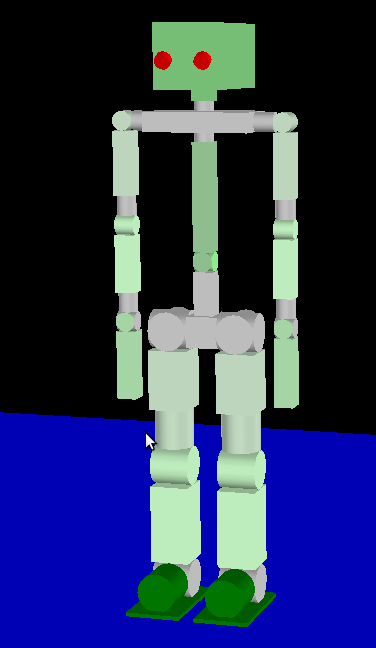
\includegraphics[width=0.3\linewidth]{Annexe1/figures/SampleHumanoid.png}
  \end{center}
  \caption{Model used for benchmarking}
  \label{fig:samplehumanoid}
\end{figure}

\begin{table*}
  \begin{center}
  \begin{tabular}{|c|c|c|l|l|l|} \hline
    Nickname &                         CPU name & Frequency &  Core number & Cache size & Distribution \\ \hline \hline
    CPU-1    & Intel(R) Core(TM) i7-2820QM CPU  & 2.3 GHz   & 8            & 8 Mb       & Ubuntu 12.04 LTS \\
    CPU-2    & Intel(R) Core2(TM) Duo E7500     & 2.8 GHz   & 1            & 3 Mb       & Ubuntu 10.04 LTS \\
    CPU-3    & Intel(R) Xeon(R) CPU E3-1240 v3  & 3.4 GHz   & 8            & 8 Mb       & Ubuntu 12.04 LTS \\
    CPU-4    & Intel(R) Atom(TM) CPU N720       & 1.6 Ghz   & 1            & 512 Kb     & Ubuntu 12.04 LTS \\ \hline 
  \end{tabular}
  \caption{CPUs used for the benchmarking. CPU-1 is a laptop, CPU-2 is one used in HRP-2, CPU-3 is a desktop, and CPU-4 is a NetPC.
CPU-2 is using only one core due to the real-time operating system recognizing only one core.}
  \label{table:CPUs}
  \end{center}
\end{table*}

\subsection{Benchmarks}
We compared the performances of \softmetapod with \softrbdl by computing the inertia matrix and the inverse dynamics on the CPUs
listed in Table ~\ref{table:CPUs}.
In each case, the library was recompiled using the GNU gcc compiler with the optimization options (-O3 -NDEBUG) 
trying to generate the code producing the best performances. The model used for benchmarking is the sample humanoid model
provided by Tokyo University in OpenHRP. The model is displayed in Fig.~\ref{fig:samplehumanoid}.
For this specific work we concentrated in two algorithms which are used in controlling a humanoid robot,
the Composite Rigid Body Algorithm (CRBA) which computes the inertia matrix, and the Recursive Newton-Euler Algorithm (RNEA)
which provides the torques necessary to counterbalance the gravity. 

Table ~\ref{tab:CPU:comparison} provides a quick view on the performance difference between \softmetapod and \softrbdl on various CPUs.
The next section will detail some aspects related to the CPUs which will try to explain that the values provided
here are to be taken cautiously and are likely to highly vary according to the CPU, the context of its overload,
the compiler and the operating system. For this reason, we provide in Table ~\ref{tab:CPU:comparison} a ratio
according to the CPU between the time provided by \softmetapod and \softrbdl. 
Note that CPU-2 corresponds to the HRP-2 real chipset with its real-time operating system. The interested user
should perform an identical comparison for its own robot to have accurate time measurement. 
Here we have put the most favorable time measurements for both algorithms.
Despite this high variability, \softmetapod is almost always better in performances than \softrbdl.

We have started some comparisons with symbolic computation libraries, but they usually imply
the use of a costly third-part software. A comparison with \softhumans on a structure similar to the model
used here gives $8.35 \mu s$ for the CRBA algorithm on CPU-1. To achieve this result on \softmetapod with CPU-1 it was necessary
to use the compiler options given in the remainder of the paper. They changed nothing for \softhumans.
As the later one does not use Eigen, this implies that, as mentionned by Featherstone, the use of
vector-based arithmetic has a strong impact when computing the inertia matrix.
Thanks to the authors of \softsymoro, and if the paper is accepted, we hope to augment the comparison with this software.

\begin{table*}
  \begin{center}
    \begin{tabular}{|c|c|p{1cm}|m{1cm}|m{1cm}|m{1cm}|m{1cm}|m{1cm}|m{1cm}|m{1cm}|} \hline
      Library                  & Algorithms &  \multicolumn{2}{|c|}{CPU-1}      & \multicolumn{2}{|c|}{CPU-2} & \multicolumn{2}{|c|}{CPU-3}  & 
      \multicolumn{2}{|c|}{CPU-4} \\ \hline \hline
                               &            &  $\mu s$ & ratio & $\mu s$  & ratio    & $\mu s$ & ratio   &  $\mu s$  & ratio \\ \hline
      \multirow{3}{*}{\softmetapod} & CRBA       &  $7.89$  & 0.77  & $12.97$  &  0.69   & $5.08$  & 0.76      & $61.06$  & 0.76 \\
                               & RNEA       &  $9.28$  & 0.97  & $13.85$  &  0.75   & $4.93$  & 0.82      & $60.98$  & 0.90 \\ \hline
      \multirow{3}{*}{\softrbdl}    & CRBA       &  $10.16$ &       & $18.59$  &         & $6.60$  &           & $79.68$  & \\
                               & RNEA       &  $9.5$   &       & $18.66$  &         & $5.99$  &           & $67.68$  & \\ \hline
    \end{tabular}
  \end{center}
  \caption{Processing time for three basic algorithms used in control of humanoid robot: Inertia matrix computation (CRBA),
    Inverse Dynamics (RNEA). The computation have been tested on 4 CPUs.}
  \label{tab:CPU:comparison}
\end{table*}

\subsection{CPUs}

The Intel company divides its chipsets into 3 categories: Core, Xeon and Atom. 
With its low power consumption and low heat dissipation the Atom processor is aimed for embedded systems. 
The first and second families are used respectively for desktop applications and high power computation. 
The Xeon Phi category is targeted for many cores applications.

\subsubsection{TurboBoost}
To speed up the performance of the Core and Xeon families their coprocessors embed
a technology that Intel names TurboBoost. It consists in increasing the CPU speed while respecting safety rules 
regarding heat dissipation and voltage. The maximum speed that can be reached is called the maximum turbo frequency.
For instance regarding Table ~\ref{tab:CPU:comparison} CPU-1 and CPU-3 can reach respectively 3.4 GHz (from 2.3 GHz) and 
3.8 Ghz (from 3.6 GHz). There is no guarantee that the maximum frequency is always reached as it depends on the
current status on the chipsets. The Atom chipsets do not have the TurboBoost technology as well as the Core2 Duo E7500 (CPU-2)
currently inside the HRP-2 humanoid robot. This is reflected by the numbers given in Table ~\ref{tab:CPU:comparison},
where the raw times are 10 times faster on Xeon chipsets than on Atom. Interestingly one would have expected
that CPU-1 with the turbo-boost would be at best near 0.9 the speed of CPU-3, as it is the ratio of their respective
Turbo-Boost frequency. This relationship is not verified between CPU-1 and CPU-3. 
In addition the description of the TurboBoost technology in the Sandy Bridge micro architecture \cite{Rotem:IEEEMicro:2012}
shows a complex pattern depending on the current overall status of the CPU.
It is worth noting that the operating system can also request TurboBoost by sending a signal (P-state request) if it detects an overloading status. 

\subsubsection{Branch prediction}
Performances depend on another key technology: branch prediction.
The chipset maintains counters to predict the branches behavior. 
Depending on the statistics of the branch, the predictor tries to guess
what will we be the most probable code to be executed by the CPU.
The code and its data are then prefetched from the memory while the CPU
is decoding the current operation.
Branch predictors can also detect cycles and save in cache intermediate variables
to avoid costly access memory.
Branch predictors is also able to indirect branch where multiple address are possible
targets.
The interest of the symbolic approach is to avoid as much as possible to make branches
in the code. It facilitates the work of the branch predictor as well as the memory pre-fetching
mechanism. This may explain why in Table ~\ref{tab:CPU:comparison} \softmetapod provides a 25-30 \% increase
in efficiency on the CRBA algorithm. 
%
\begin{table*}  
  \begin{center}
    %\begin{footnotesize}
      \begin{tabular}{|c|r|r|r|r|r|r|r|r|r|} \hline
        Library  &             Ir &       I1mr & ILmr  &            Dr &      D1mr &  DLmr &            Dw &       D1mw &  DLmw \\ \hline
        \softrbdl    &  8,295,618,744 &     39,643 & 3,995 & 3,447,245,971 & 2,936,723 & 7,322 & 1,617,919,310 &    607,848 & 3,447  \\
        \softmetapod &  4,529,574,180 & 69,802,287 & 2,722 & 2,154,169,130 & 9,709,886 & 5,040 & 1,034,216,699 & 27,501,390 & 1,136  \\ \hline
      \end{tabular}\\     
      \caption{{\bf Ir}: Number of executed instructions, {\bf I1m1r}: Instruction read misses for cache L1, {\bf ILmr}: Instruction read misses for Last Level cache,
        {\bf Dr}: Number of cache read, {\bf D1mr}: Data read misses for cache L1, {\bf DLmr}: Data read misses for Last Level cache,
        {\bf Dw}: Number of cache write, {\bf D1mw}: Data write misses for cache L1, {\bf DLmw}: Data write misses for Last Level cache.
      Tests realized on CPU-1}
      \label{tab:cache:valgrind}      
  \end{center}
\end{table*}
%
\begin{table*}  
  \begin{center}
    \begin{tabular}{|c|r|r|r|r|} \hline
      Library &           Bc &       Bcm &         Bi &     Bim \\ \hline
      \softrbdl    &  245,662,040 & 7,604,170 & 45,177,857 & 269,654 \\
      \softmetapod &   98,901,411 &   977,079 & 14,105,063 &     726 \\ \hline
    \end{tabular}
    \caption{ {\bf Bc}: Conditional branches executed, {\bf Bcm}: conditional branches mispredicted,
    {\bf Bi}: Indirect branches executed {\bf Bim}: indirect branches mispredicted. Tests realized on CPU-1}
    \label{tab:branch:valgrind}
  \end{center}
\end{table*}
%
Unfortunately chipsets providers, in general, do not give a detailed description of their branch predictors.
For this reason, users have usually to reverse engineer the behavior of the chipset in order
to create branch predictor aware compilers \cite{wang:iiswc:2011,Uzelac:ispass:2009}.
We used Valgrind framework to analyse cache access and branch prediction.
The result is compiled in Table ~\ref{tab:cache:valgrind} and in Table ~\ref{tab:branch:valgrind}.
From Table ~\ref{tab:cache:valgrind} \softmetapod is doing more misprediction than \softrbdl for the Level 1 cache both for instruction and data,
but less for the last level cache. As a last level misprediction implies a memory access, with the slower bus frequency it is the most costly.
Therefore this result is in favor of \softmetapod. 
In addition Table ~\ref{tab:branch:valgrind} shows clearly that branch misprediction is far lower for \softmetapod than for \softrbdl.

\subsubsection{Compiler}
The importance of the compiling options differs according to the library and the CPUs.
It was particularly strong on the Atom chipset with a gain of $20 \mu s$ for \softmetapod and \softrbdl. 
On \softrbdl, the impact of compiling option was null on CPU-1 and CPU-3 whereas it is improved by 10 \% on \softmetapod.
The compiler options used to exploit vector-based arithmetic and loop optimizations are
\footnote{We kindly invite the interested reader to follow the gcc manual for a more detailed explanation of the
options}:
\begin{verbatim}
-msse -msse2 -msse3 -march=corei7 -mfpmath=sse 
-fivopts -ftree-loop-im -fipa-pta
\end{verbatim}
In addition during the linking phase it is possible to strip out useless code and perform 
whole-program optimization with the following optionx:
\begin{verbatim}
-fwhole-program
\end{verbatim}
Again the static structure of the code generated through \softmetapod simplifies the work
of optimization strategies applied by the compiler (here gcc).






